\documentclass[10pt,a4paper]{article}
\usepackage[utf8]{inputenc}
\usepackage[T1]{fontenc}
\usepackage[a4paper,top=1.5cm,bottom=1.5cm,left=1.5cm,right=1.5cm]{geometry}
\usepackage{amsmath}
\usepackage{amssymb}
\usepackage{tikz}
\usetikzlibrary{calc,patterns}
\usepackage[dvipsnames,svgnames]{xcolor}
\usepackage{booktabs}
\usepackage{tabularx}
\usepackage{array}
\usepackage[bookmarks=false]{hyperref}

\title{Rubrik Nilai Tugas Minggu 1 : Sistem Bilangan Real}
\author{Matematika untuk Sistem Informasi}
\date{}

\newenvironment{rubrik}{%
  \noindent
  \tabularx{\textwidth}{@{}>{\raggedright\arraybackslash}p{2.2cm}>{\raggedright\arraybackslash}X>{\centering\arraybackslash}p{1.1cm}>{\centering\arraybackslash}p{1.4cm}@{}}
  \toprule
  \textbf{Kriteria} & \textbf{Deskriptor} & \textbf{Maks} & \textbf{Skor} \\
  \midrule
}{%
  \bottomrule
  \endtabularx\par
}
\newcommand{\butir}[1]{\par\vspace{0.75em}\noindent\textbf{#1}\par\vspace{0.35em}}

\begin{document}
\maketitle

\noindent
Nama: \underline{\hspace{7.2cm}} \quad NIM: \underline{\hspace{4.2cm}}

\section*{Petunjuk penilai}
\begin{itemize}
  \item Tiap butir maksimum 100. Nilai tugas adalah rata-rata skor butir.
  \item Ketentuan skor:\par
  {\small
  \setlength{\tabcolsep}{4pt}%
  \begin{tabularx}{\linewidth}{@{}>{\raggedright\arraybackslash}p{2.1cm}>{\centering\arraybackslash}p{1.1cm}>{\raggedright\arraybackslash}X@{}}
  \toprule
  \textbf{Kriteria} & \textbf{Maks} & \textbf{Ketentuan} \\
  \midrule
  Langkah & 50 & Jika langkah terbaca dan tidak seluruhnya salah, skor minimal 25. Skor di bawah 25 hanya bila langkah salah total, tidak dimengerti, atau tidak terbaca. \\
  Jawaban & 30 & Harus ada dan benar. Skor hanya 0 atau nilai penuh. \\
  Penyajian & 20 & Harus ada dan benar. Skor hanya 0 atau nilai penuh. \\
  \bottomrule
  \end{tabularx}}
\end{itemize}

\butir{Butir 1. $2 - 3x \leq 12$ (100 poin)}
\begin{rubrik}
Langkah &
Kurangi kedua ruas, lalu kalikan dengan bilangan negatif sehingga tanda pertidaksamaan berbalik. &
50 & \\
Jawaban &
$\mathrm{HP} = \bigl[-\frac{10}{3}, \infty\bigr)$. &
30 & \\
Penyajian &
Garis bilangan: titik penuh di $-\frac{10}{3}$, arsiran ke kanan.\par\vspace{0.4em}
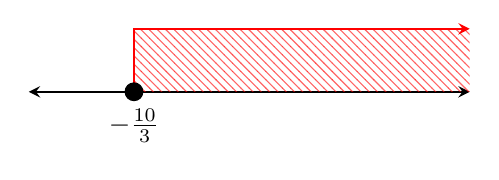
\begin{tikzpicture}[scale=0.8]
\draw[thick,stealth-stealth] (-5,0)--(2,0);
\draw[thick,-stealth,Red] (-3.33,0)--(-3.33,1)--(2,1);
\path[pattern=north west lines,opacity=.6,pattern color=Red] (-3.33,0)--(-3.33,1)--(2,1)--(2,0)--cycle;
\filldraw[black,fill=black] (-3.33,0) node[below,yshift=-.1cm] {$-\frac{10}{3}$} circle (0.4em);
\end{tikzpicture} &
20 & \\
\midrule
\multicolumn{2}{r}{\textbf{Jumlah}} & 100 & \\
\end{rubrik}

\butir{Butir 2. $3x - 5 < 4x - 6$ (100 poin)}
\begin{rubrik}
Langkah &
Kumpulkan suku $x$ pada satu ruas dan kalikan dengan $-1$ sehingga tanda berbalik. &
50 & \\
Jawaban &
$\mathrm{HP} = (1, \infty)$. &
30 & \\
Penyajian &
Garis bilangan: titik kosong di $1$, arsiran ke kanan.\par\vspace{0.4em}
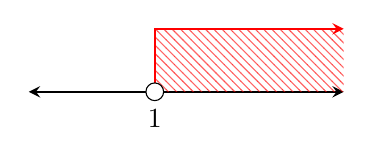
\begin{tikzpicture}[scale=0.8]
\draw[thick,stealth-stealth] (-1,0)--(4,0);
\draw[thick,-stealth,Red] (1,0)--(1,1)--(4,1);
\path[pattern=north west lines,opacity=.6,pattern color=Red] (1,0)--(1,1)--(4,1)--(4,0)--cycle;
\filldraw[black,fill=white] (1,0) node[below,yshift=-.1cm] {$1$} circle (0.4em);
\end{tikzpicture} &
20 & \\
\midrule
\multicolumn{2}{r}{\textbf{Jumlah}} & 100 & \\
\end{rubrik}

\butir{Butir 3. $-3 \leq 1 - 6x < 4$ (100 poin)}
\begin{rubrik}
Langkah &
Operasi yang sama dikenakan pada ketiga bagian; pembagian dengan negatif membalik kedua tanda. &
50 & \\
Jawaban &
$\mathrm{HP} = \bigl(-\frac{1}{2}, \frac{2}{3}\bigr]$. &
30 & \\
Penyajian &
Garis bilangan: kosong di $-\frac{1}{2}$, penuh di $\frac{2}{3}$, arsiran di antaranya.\par\vspace{0.4em}
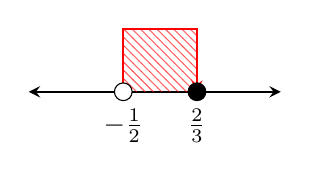
\begin{tikzpicture}[scale=0.8]
\draw[thick,stealth-stealth] (-2,0)--(2,0);
\draw[thick,-stealth,Red] (-0.5,0)--(-0.5,1)--(0.67,1)--(0.67,0);
\path[pattern=north west lines,opacity=.6,pattern color=Red] (-0.5,0)--(-0.5,1)--(0.67,1)--(0.67,0)--cycle;
\filldraw[black,fill=white] (-0.5,0) node[below,yshift=-.1cm] {$-\frac{1}{2}$} circle (0.4em);
\filldraw[black,fill=black] (0.67,0) node[below,yshift=-.1cm] {$\frac{2}{3}$} circle (0.4em);
\end{tikzpicture} &
20 & \\
\midrule
\multicolumn{2}{r}{\textbf{Jumlah}} & 100 & \\
\end{rubrik}

\butir{Butir 4. $2x^2 - 5x - 3 < 0$ (100 poin)}
\begin{rubrik}
Langkah &
Bentuk baku, titik kritis $x = -\frac{1}{2}$ dan $x = 3$, lalu analisis tanda pada tiap selang. &
50 & \\
Jawaban &
$\mathrm{HP} = \bigl(-\frac{1}{2}, 3\bigr)$. &
30 & \\
Penyajian &
Garis bilangan: kedua titik kosong, arsiran hanya di antara kedua akar.\par\vspace{0.4em}
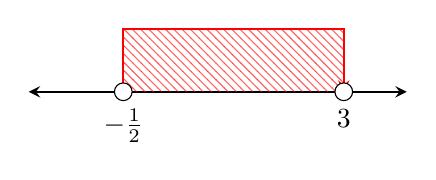
\begin{tikzpicture}[scale=0.8]
\draw[thick,stealth-stealth] (-2,0)--(4,0);
\draw[thick,-stealth,Red] (-0.5,0)--(-0.5,1)--(3,1)--(3,0);
\path[pattern=north west lines,opacity=.6,pattern color=Red] (-0.5,0)--(-0.5,1)--(3,1)--(3,0)--cycle;
\filldraw[black,fill=white] (-0.5,0) node[below,yshift=-.1cm] {$-\frac{1}{2}$} circle (0.4em);
\filldraw[black,fill=white] (3,0) node[below,yshift=-.1cm] {$3$} circle (0.4em);
\end{tikzpicture} &
20 & \\
\midrule
\multicolumn{2}{r}{\textbf{Jumlah}} & 100 & \\
\end{rubrik}

\butir{Butir 5. $x^2 - 5x - 6 \leq 0$ (100 poin)}
\begin{rubrik}
Langkah &
Bentuk baku, titik kritis $x = -1$ dan $x = 6$, lalu analisis tanda. &
50 & \\
Jawaban &
$\mathrm{HP} = [-1, 6]$. &
30 & \\
Penyajian &
Garis bilangan: kedua titik penuh karena tanda $\leq$, arsiran di antaranya.\par\vspace{0.4em}
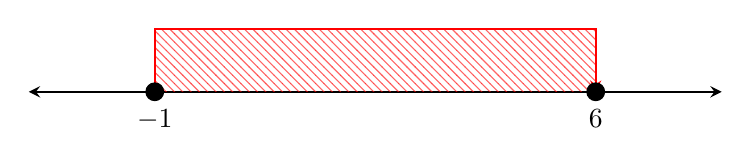
\begin{tikzpicture}[scale=0.8]
\draw[thick,stealth-stealth] (-3,0)--(8,0);
\draw[thick,-stealth,Red] (-1,0)--(-1,1)--(6,1)--(6,0);
\path[pattern=north west lines,opacity=.6,pattern color=Red] (-1,0)--(-1,1)--(6,1)--(6,0)--cycle;
\filldraw[black,fill=black] (-1,0) node[below,yshift=-.1cm] {$-1$} circle (0.4em);
\filldraw[black,fill=black] (6,0) node[below,yshift=-.1cm] {$6$} circle (0.4em);
\end{tikzpicture} &
20 & \\
\midrule
\multicolumn{2}{r}{\textbf{Jumlah}} & 100 & \\
\end{rubrik}

\butir{Butir 6. $\displaystyle \frac{1}{x+1} < \frac{2}{3x-1}$ (100 poin)}
\begin{rubrik}
Langkah &
Pindah ke satu ruas, titik kritis termasuk nol penyebut $x = -1$ dan $x = \frac{1}{3}$, lalu analisis tanda. &
50 & \\
Jawaban &
$\mathrm{HP} = (-\infty, -1) \cup \bigl(\frac{1}{3}, 3\bigr)$. &
30 & \\
Penyajian &
Garis bilangan: titik kritis terbuka, penyebut yang nol tidak masuk HP.\par\vspace{0.4em}
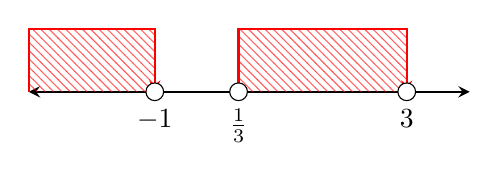
\begin{tikzpicture}[scale=0.8]
\draw[thick,stealth-stealth] (-3,0)--(4,0);
\draw[thick,-stealth,Red] (-3,0)--(-3,1)--(-1,1)--(-1,0);
\draw[thick,-stealth,Red] (0.33,0)--(0.33,1)--(3,1)--(3,0);
\path[pattern=north west lines,opacity=.6,pattern color=Red] (-3,0)--(-3,1)--(-1,1)--(-1,0)--cycle;
\path[pattern=north west lines,opacity=.6,pattern color=Red] (0.33,0)--(0.33,1)--(3,1)--(3,0)--cycle;
\filldraw[black,fill=white] (-1,0) node[below,yshift=-.1cm] {$-1$} circle (0.4em);
\filldraw[black,fill=white] (0.33,0) node[below,yshift=-.1cm] {$\frac{1}{3}$} circle (0.4em);
\filldraw[black,fill=white] (3,0) node[below,yshift=-.1cm] {$3$} circle (0.4em);
\end{tikzpicture} &
20 & \\
\midrule
\multicolumn{2}{r}{\textbf{Jumlah}} & 100 & \\
\end{rubrik}

\butir{Butir 7. $\displaystyle \frac{x+2}{x+4} < \frac{x-1}{x-2}$ (100 poin)}
\begin{rubrik}
Langkah &
Pindah ke satu ruas, titik kritis termasuk $x = -4$ dan $x = 2$, lalu analisis tanda. &
50 & \\
Jawaban &
$\mathrm{HP} = (-4, 0) \cup (2, \infty)$. &
30 & \\
Penyajian &
Garis bilangan: selang terbuka pada batas dan pada nol penyebut.\par\vspace{0.4em}
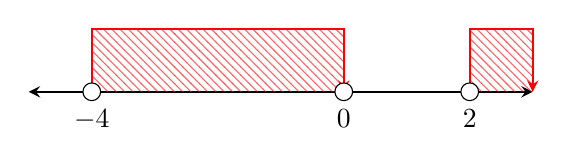
\begin{tikzpicture}[scale=0.8]
\draw[thick,stealth-stealth] (-5,0)--(3,0);
\draw[thick,-stealth,Red] (-4,0)--(-4,1)--(0,1)--(0,0);
\draw[thick,-stealth,Red] (2,0)--(2,1)--(3,1)--(3,0);
\path[pattern=north west lines,opacity=.6,pattern color=Red] (-4,0)--(-4,1)--(0,1)--(0,0)--cycle;
\path[pattern=north west lines,opacity=.6,pattern color=Red] (2,0)--(2,1)--(3,1)--(3,0)--cycle;
\filldraw[black,fill=white] (-4,0) node[below,yshift=-.1cm] {$-4$} circle (0.4em);
\filldraw[black,fill=white] (0,0) node[below,yshift=-.1cm] {$0$} circle (0.4em);
\filldraw[black,fill=white] (2,0) node[below,yshift=-.1cm] {$2$} circle (0.4em);
\end{tikzpicture} &
20 & \\
\midrule
\multicolumn{2}{r}{\textbf{Jumlah}} & 100 & \\
\end{rubrik}

\section*{Rekap skor}
\noindent
\begin{tabular}{@{}lr@{}}
\toprule
Butir & Skor \\
\midrule
1 & \\
2 & \\
3 & \\
4 & \\
5 & \\
6 & \\
7 & \\
\midrule
Rata-rata = jumlah skor / 7 (maksimum 100) & \\
\bottomrule
\end{tabular}

\end{document}
